\section{Such-Seite [M]}
Auf der Such-Seite können Benutzer*innen nach bestimmten Ausstellungen suchen. Dabei kann nach dem Titel einer Ausstellung, nach dem Ersteller einer Ausstellung oder nach bestimmten Kategorien gefiltert werden. Bei der Suche handelt es sich um eine Vorschlagssuche, auch Typeahead-Suche genannt. Dabei werden schon während der Benutzereingabe mögliche Suchergebnisse angezeigt.

\begin{figure} [h t]
  \centering
  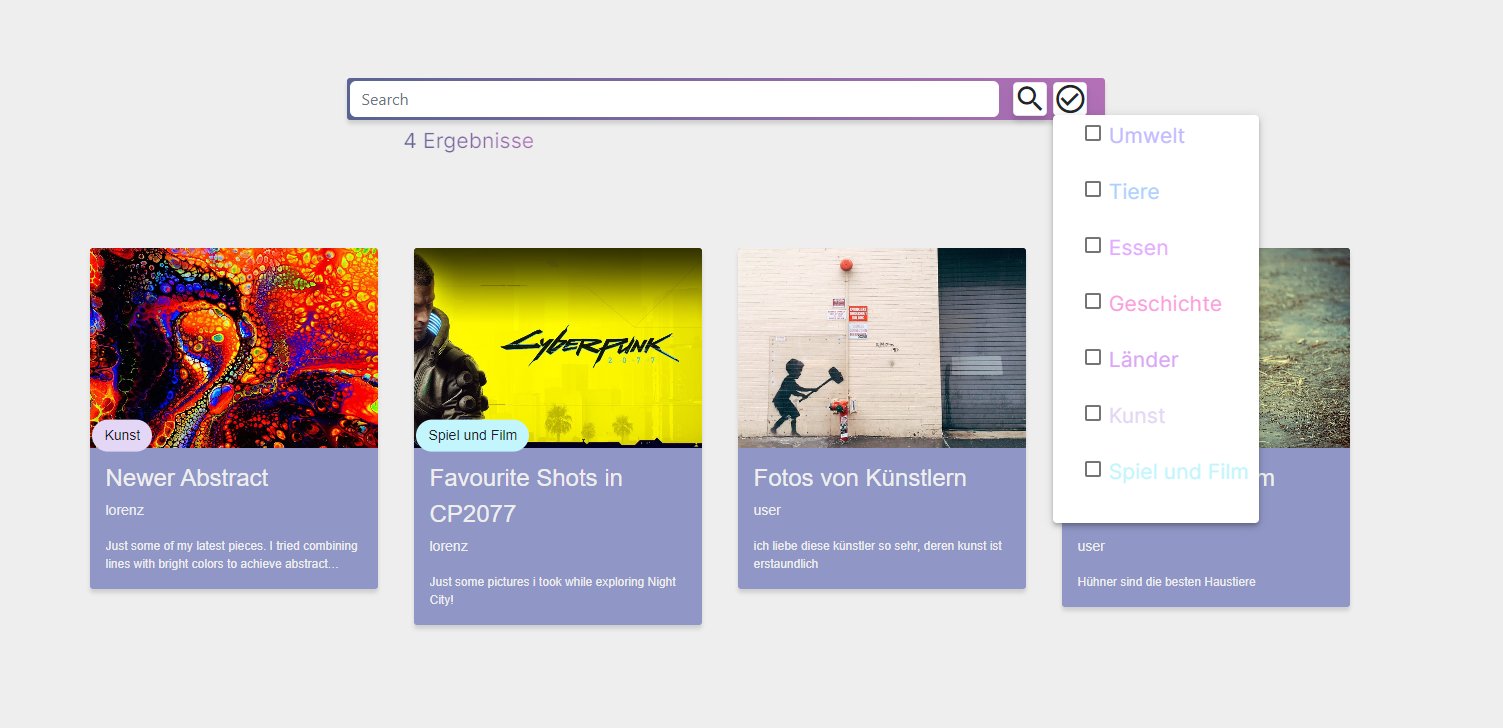
\includegraphics[scale=0.55]{pics/search-page.png}
  \caption{Search-Page}
  \label{fig:impl:search-page}
\end{figure}

Falls der*die Nutzer*in noch keine Suche gestartet hat, werden ihm alle Ausstellungen angezeigt. Diese werden über die Datenbank und den HTTP-Service (siehe Angular Services \ref{httpService}) in die Benutzeroberfläche geladen. 

Der*Die Benutzer*in kann in einem Eingabefeld einen beliebigen Suchbegriff eingeben. Nach jedem Buchstaben wird über einen Event-Listener (sieh Event-Listener \ref{txt:glos:event-listener}) diese Eingabe überprüft. 

\begin{lstlisting}[caption={Eingabefeld},language=HTML]
    
<input type="search" class="form-control rounded" placeholder="Search" #input (keyup)="keyUp$.next(input.value)">
    
\end{lstlisting}

Anschließend wird die Logik der Suche implementiert. Um mehrere Operatoren in die Suchfunktion zu integrieren, wird eine Pipe (siehe \ref{txt:glos:Pipes}) benötigt. Anschließend wird ein Filter angewendet, um erst dann ein Suchergebnis zu liefern, wenn der*die Benutzer*in mindestens 3 Buchstaben in das Suchfeld eingegeben hat. Damit nicht nach jeder Tastaturabgabe eine Anfrage an die Datenbank geschickt wird, wird der Operator \emph{debounceTime} angewandt. Dabei wird erst dann eine Anfrage gesendet, nachdem der*die Benutzer*in eine gewisse Zeit nichts mehr in das Eingabefeld geschrieben hat. Durch die Methode \emph{distinctUntilChanged} werden außerdem keine unnötigen Anfragen an den Server gesendet, falls sich der Suchbegriff nicht geändert hat. Da hierbei eine Subscription in einer Subscription vorhanden ist, wird ohne einen Flatting-Operator wieder der gleiche eingegebene Suchbegriff zurückgeliefert und keine Suchergebnisse. Daher wird der Operator \emph{swichtMap} verwendet, der zusätzlich alle Anfragen an den Server abbricht, sobald sich die Sucheingabe, durch Einwirken des*der Benutzers*in, ändert. Somit können die vom Server gesendeten Suchergebnisse direkt in ein Array von Ausstellungsstücken gespeichert werden. Dabei werden, wie bei einer Vorschlagssuche, die gefilterten Ausstellungen dem Benutzer angezeigt und bei Veränderung des Suchbegriffs aktualisiert.

\begin{lstlisting}[caption={Die Such-Pipe mit den Filter-Operatoren},language=HTML]

    this.keyUp$.pipe(
        filter(term => term.length >= 3),
        debounceTime(500),
        distinctUntilChanged(),
        switchMap(searchTerm => this.galleryService.getAllSearch(searchTerm)),
      ).subscribe(exhibitions => this.searchResults = exhibitions)
        
\end{lstlisting}

\subsection{Filtern mittels Kategorien}

Zusätzlich zu der Suche über das Eingabefeld, kann der*die Benutzer*innen Ausstellungen zusätzlich filtern. Eine Ausstellung kann bei ihrer Konfiguration, keiner, einer oder mehrerer Kategorien zugeordnet werden. Alle Kategorien werden in einem Menü aufgelistet und können durch eine Checkbox für das Filtern ausgewählt werden. Beim Auswählen einer Kategorie wird diese einem Array aus Kategorien hinzugefügt. Falls der*die Benutzer*in eine Kategorie wieder abwählt, wird diese vom Array entfernt.   


\begin{lstlisting}[caption={Auswählen und Abwählen der Kategorien},language=HTML]

    addCategory(id: number){
        if(!this.selectedCategories.find(c => c == id)){
            this.selectedCategories.push(id)
        }else{
          for( var i = 0; i < this.selectedCategories.length; i++){
            if ( this.selectedCategories[i] === id) {
              this.selectedCategories.splice(i, 1);
            }
          }
        }
    }
        
\end{lstlisting}

Beim Schließen des Menüs wird automatisch nach den ausgewählten Kategorien gefiltert.


\begin{lstlisting}[caption={Filter von Kategorien anwenden},language=HTML]

    onMenuClose(){
        this.filter_icon = "filter_alt";
        let searchString = "";
        for(let i = 0; i < this.selectedCategories.length; i++){
          searchString += this.selectedCategories[i] + ","
        }
        if(this.selectedCategories.length > 0){
          this.galleryService.getExhibitonByIds(searchString).subscribe(e => {
            this.searchResults = e
          })
        }else{
          this.galleryService.getAllExhibitions().subscribe(res => this.searchResults = res);
        }
    }
\end{lstlisting}



\subsection{Erledigte User-Stories [L]}
In dem Entwicklungsprozess der Suchseite wurden folgende User-Stories vollendet:
\begin{compactitem}
  \item Als Besucher*in möchte ich eine Suchseite haben, um Designer*innen und deren Ausstellungen finden zu können. Ich will, dass die Suchseite durch einen CTA-Button aufrufbar ist. Außerdem sollen auf der Suchseite unterschiedliche Optionen zur Suche sein. Das Suchergebnis soll ansprechend dargestellt werden.
  \item Als Besucher*in der Webseite will ich beim Suchen filtern können, um für mich die relevantesten Ergebnisse zu bekommen. Die Filtermöglichkeiten sollen Tags, Favoriten und das Erstellungsdatum beinhalten.
\end{compactitem}